\chapter{Propuesta}

\section{Metodolog\'ia utilizada}
Para el desarrollo de esta app, usar\'e una metodolog\'ia \textit{\'agil} tipo \textbf{SCRUM}. He decidido usar esta porque me permite corregir fallos en la velocidad de dise\~no y/o planificaci\'on de forma eficiente y sin da\~nar el producto final.

Las reuniones con la tutora ser\'an las \textit{sprint reviews}.

\section{Temporizaci\'on}
La temporizaci\'on se realiz\'o el d\'ia 25 de marzo de 2025. La entrega del producto (este TFG) est\'a prevista para el 16 de junio de 2025, es decir, 83 d\'ias, o lo que es lo mismo, casi 12 semanas. Si un sprint dura 2 semanas, habr\'a 6 sprints hasta la entrega final.

La iteraci\'on 0 se dedicar\'a al dise\~no de pantallas y al repaso de las funcionalidades de la app. La idea inicial es dividir la app en varios m\'odulos y centrar cada sprint en uno de ellos:

\begin{itemize}
  \item Diagramas de la app y ejercicios
  \item Rutinas, usuarios y sesi\'on
  \item Datos que ingresa el usuario
  \item Flujo de entrenamiento
  \item Inteligencia Artificial (IA)
  \item Smartwatch
\end{itemize}

\section{Seguimiento del desarrollo}

\subsection{Iteraci\'on 0}
En esta primera iteraci\'on me cent\'re en completar los dise\~nos de la app, priorizando su accesibilidad. Tambi\'en concret\'e el \textit{product backlog}, compuesto por 41 historias de usuario. A pesar de trabajar con SCRUM se realizarán todos los diseños para concretar al tutor la idea a desarrollar en este TFG.
Algunas incluyen tareas secundarias:

\begin{description}
  \item[\textbf{SCRUM-1}] Registrar peso por d\'ia
  \item[\textbf{SCRUM-2}] Establecer peso objetivo
  \item[\textbf{SCRUM-3}] Insertar/Borrar/Modificar ejercicio de la lista de ejercicios
  \item[\textbf{SCRUM-4}] Buscar rutina en la lista del usuario
  \item[\textbf{SCRUM-5}] Sustituir un ejercicio por otro en la rutina
  \item[\textbf{SCRUM-6}] Insertar/Borrar/Modificar rutina
  \item[\textbf{SCRUM-7}] Poner una meta en cada ejercicio
  \item[\textbf{SCRUM-8}] Hacer grafica de los datos de los ejercicios
  \item[\textbf{SCRUM-9}] Revisar datos para ver si el descanso es necesario
  \item[\textbf{SCRUM-10}] Ense\~nar datos de una rutina a descargar
  \item[\textbf{SCRUM-11}] Compartir mi rutina
  \item[\textbf{SCRUM-12}] Guardar las repeticiones y series de todos los ejercicios de un entrenamiento
  \item[\textbf{SCRUM-13}] Valorar el entrenamiento en base a la marca actual y la meta del usuario
  \item[\textbf{SCRUM-14}] Monitorizar pulso en tiempo real
  \item[\textbf{SCRUM-15}] Medir pulso en reposo y compararlo con datos de ejercicios
  \item[\textbf{SCRUM-16}] Avisar de anomal\'ias en el pulso de forma suave
  \item[\textbf{SCRUM-17}] Obtener calor\'ias quemadas
  \item[\textbf{SCRUM-18}] Comprobar el equilibrio nervioso del usuario
  \item[\textbf{SCRUM-19}] Realizar el flujo del entrenamiento
  \item[\textbf{SCRUM-20}] Conectar con la IA para iniciar di\'alogo
  \item[\textbf{SCRUM-21}] Crear/Borrar usuario
  \item[\textbf{SCRUM-22}] Resumir datos
  \item[\textbf{SCRUM-23}] Iniciar/Cerrar sesi\'on
  \item[\textbf{SCRUM-24}] Medir SpO2
  \item[\textbf{SCRUM-25}] Interpretar constantes
  \item[\textbf{SCRUM-26}] Buscar ejercicios en la lista de ejercicios
  \item[\textbf{SCRUM-27}] Hacer la IU de la lista de los ejercicios
  \item[\textbf{SCRUM-28}] Hacer la IU de creación de ejercicio
  \item[\textbf{SCRUM-29}] Pop up de confirmación
  \item[\textbf{SCRUM-30}] Hacer IU de datos ejercicio
  \item[\textbf{SCRUM-31}] Crear IU de la lista de las rutinas
  \item[\textbf{SCRUM-32}] Crear IU de pantalla inicial
  \item[\textbf{SCRUM-33}] Crear IU menú principal
  \item[\textbf{SCRUM-34}] Crear IU datos rutinas
  \item[\textbf{SCRUM-35}] IU lista ejercicios de rutina modificable
  \item[\textbf{SCRUM-36}] Crear IU para crear rutina
  \item[\textbf{SCRUM-36}] Detectar metas cumplidas despues del entrenamiento
  \item[\textbf{SCRUM-37}] Crear IU del perfil del usuario
  \item[\textbf{SCRUM-38}] Detectar metas cumplidas en los ejercicios despues del entrenamiento
  \item[\textbf{SCRUM-39}] Buscar rutinas para descargar
  \item[\textbf{SCRUM-40}] IU del pop up de resumir datos
  \item[\textbf{SCRUM-41}] IU desplegable rutina
  
\end{description}

A continuación se muestran los diseños creados en esta iteración:

\textbf{Inicio de sesion y crear usuario}

\begin{figure}[H]
   \centering
    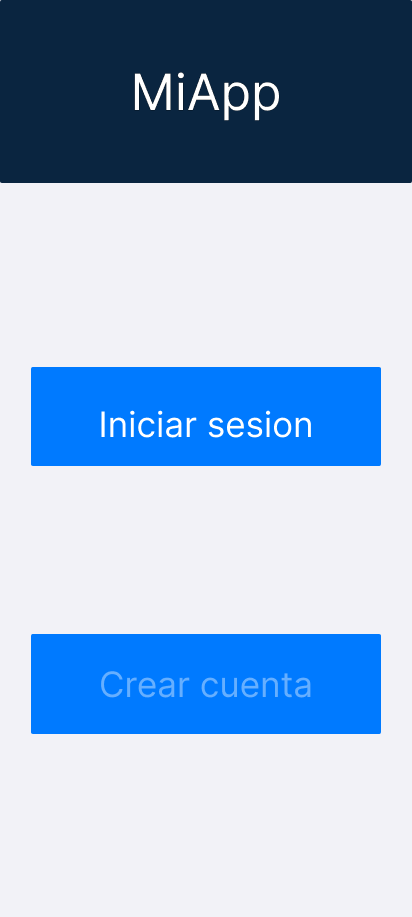
\includegraphics[width=0.6\textwidth]{fotos/Frame 22.png}
    \caption{Pagina inicial}
    \label{fig:Pagina inicial}
\end{figure}
\begin{figure}[H]
   \centering
    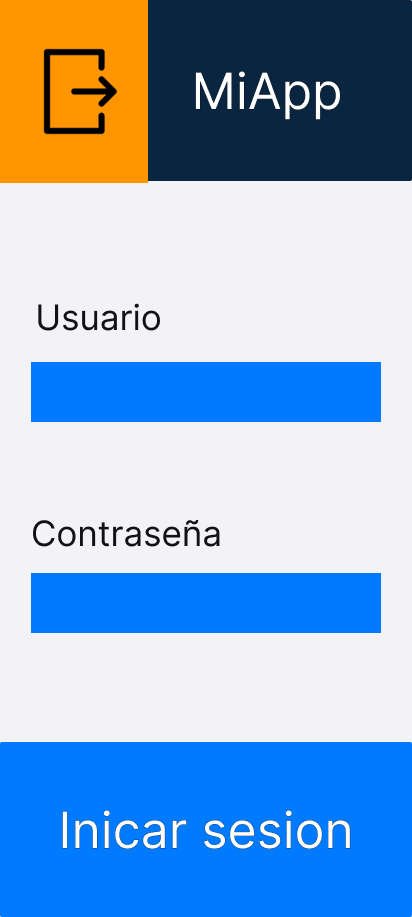
\includegraphics[width=0.6\textwidth]{fotos/Frame 22-1.png}
    \caption{Inicio de sesion}
    \label{fig:Inicio de sesion}
\end{figure}
\begin{figure}[H]
   \centering
    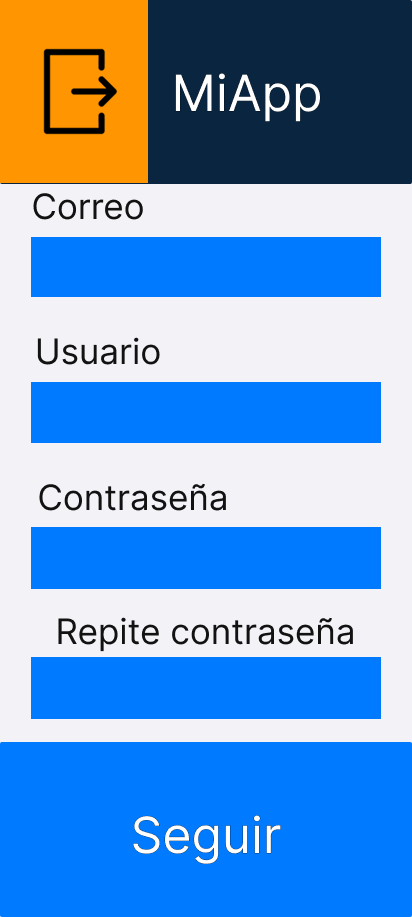
\includegraphics[width=0.6\textwidth]{fotos/Frame 24.png}
    \caption{Crear cuenta 1}
    \label{fig:Crear cuenta 1}
\end{figure}
\begin{figure}[H]
   \centering
    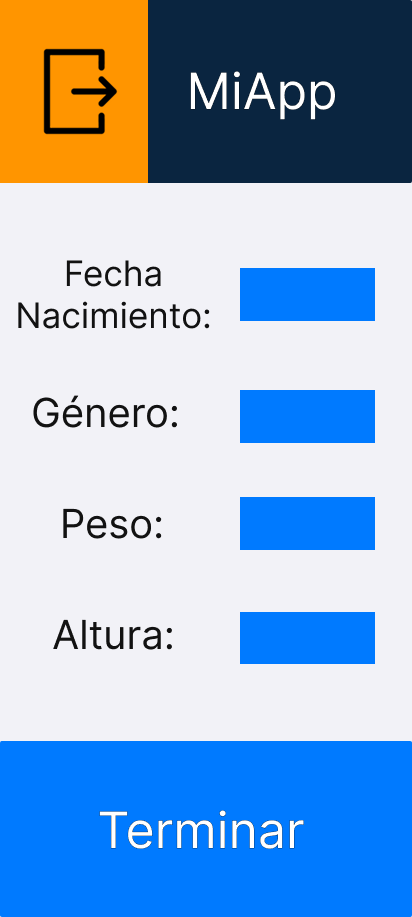
\includegraphics[width=0.6\textwidth]{fotos/Frame 25.png}
    \caption{Crear cuenta 2}
    \label{fig:Crear cuenta 2}
\end{figure}

\textbf{Menu principal}

\begin{figure}[H]
   \centering
    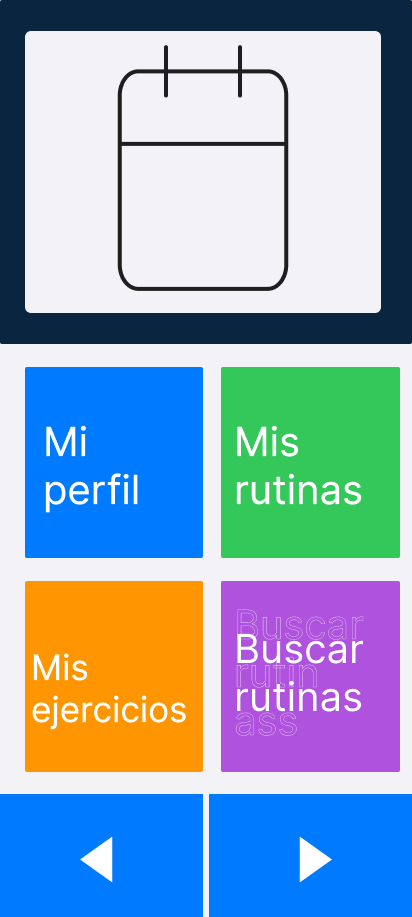
\includegraphics[width=0.6\textwidth]{fotos/Frame 30.png}
    \caption{Menu principal}
    \label{fig:Menu principal}
\end{figure}

\textbf{Lista ejercicios del usuario}

\begin{figure}[H]
   \centering
    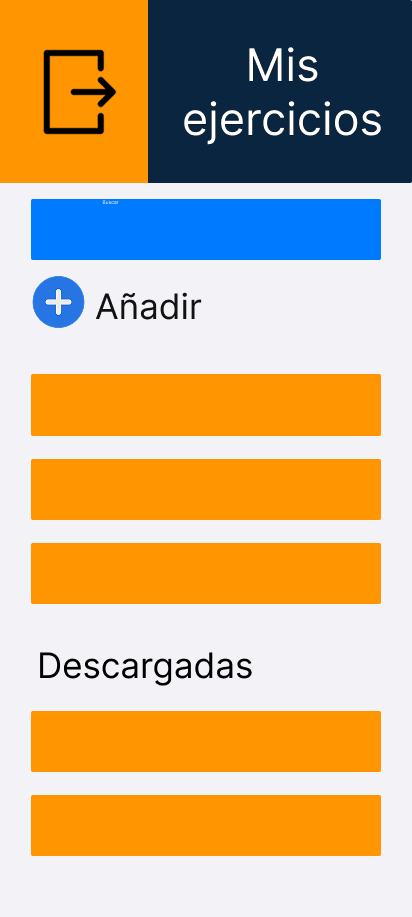
\includegraphics[width=0.6\textwidth]{fotos/Frame 40.png}
    \caption{Lista ejercicios}
    \label{fig:Lista ejercicios}
\end{figure}
\begin{figure}[H]
   \centering
    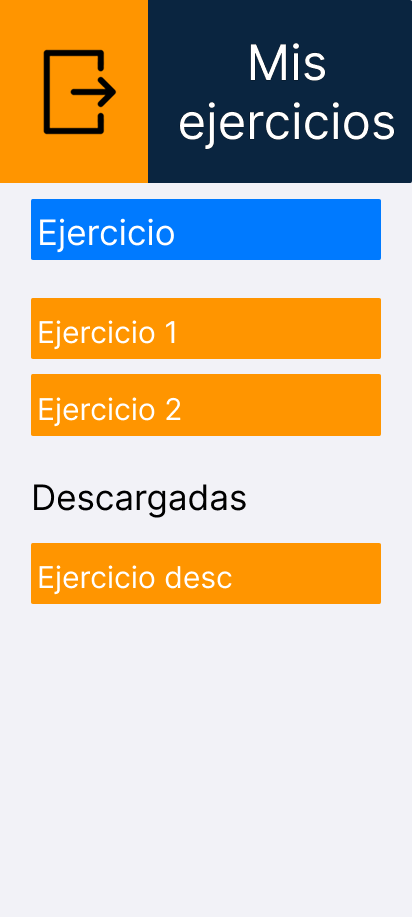
\includegraphics[width=0.6\textwidth]{fotos/Frame 41.png}
    \caption{Lista ejercicios filtrada}
    \label{fig:Lista ejercicios filtrada}
\end{figure}
\begin{figure}[H]
   \centering
    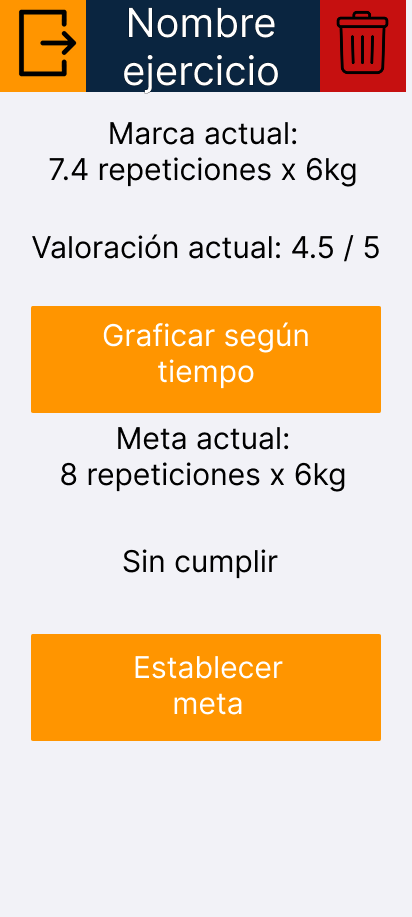
\includegraphics[width=0.6\textwidth]{fotos/Frame 42.png}
    \caption{Datos ejercicio}
    \label{fig:Datos ejercicio}
\end{figure}
\begin{figure}[H]
   \centering
    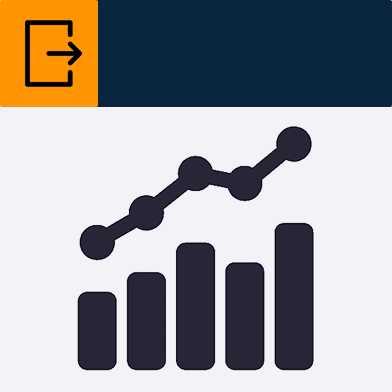
\includegraphics[width=0.6\textwidth]{fotos/Frame 43.png}
    \caption{Pop up graficar segun tiempo}
    \label{fig:Pop up graficar segun tiempo}
\end{figure}
\begin{figure}[H]
   \centering
    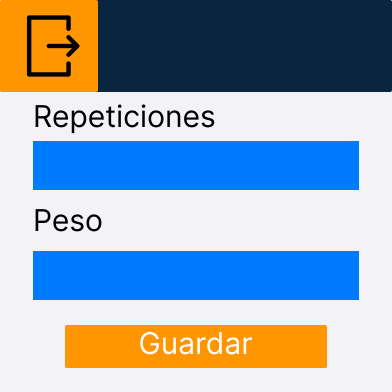
\includegraphics[width=0.6\textwidth]{fotos/Frame 45.png}
    \caption{Pop up establecer meta}
    \label{fig:Pop up establecer meta}
\end{figure}
\begin{figure}[H]
   \centering
    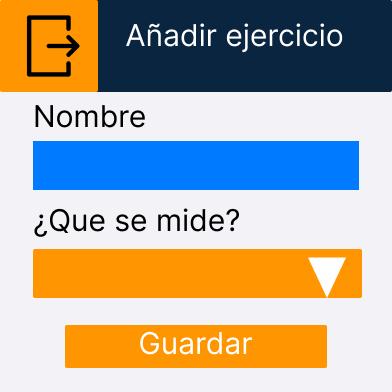
\includegraphics[width=0.6\textwidth]{fotos/Frame 64.png}
    \caption{Pop up crear ejercicio}
    \label{fig:Pop up crear ejercicio}
\end{figure}

\textbf{Lista rutinas}

\begin{figure}[H]
   \centering
    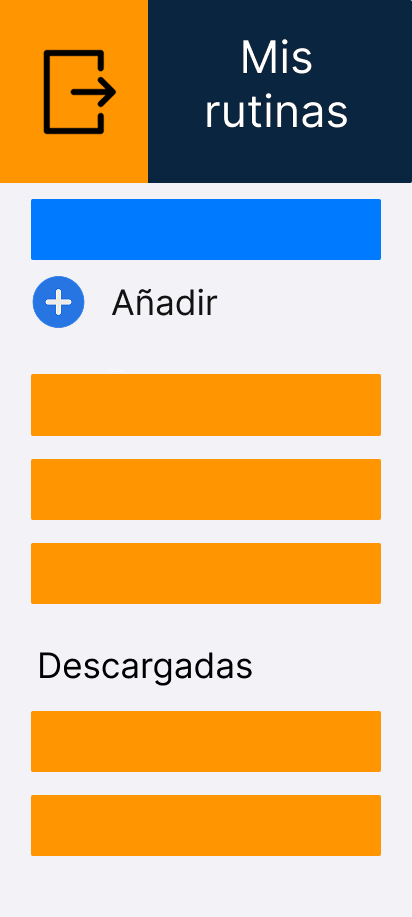
\includegraphics[width=0.6\textwidth]{fotos/Frame 46.png}
    \caption{Lista rutinas}
    \label{fig:Lista rutinas}
\end{figure}
\begin{figure}[H]
   \centering
    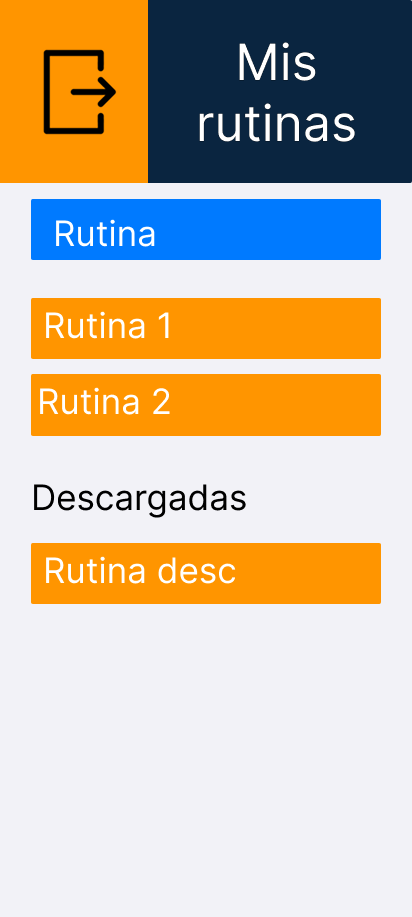
\includegraphics[width=0.6\textwidth]{fotos/Frame 47.png}
    \caption{Lista rutinas filtradas}
    \label{fig:Lista rutinas filtradas}
\end{figure}
\begin{figure}[H]
   \centering
    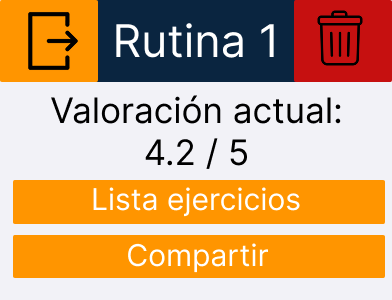
\includegraphics[width=0.6\textwidth]{fotos/Frame 48.png}
    \caption{Datos rutina modificable}
    \label{fig:Datos rutina modificable}
\end{figure}
\begin{figure}[H]
   \centering
    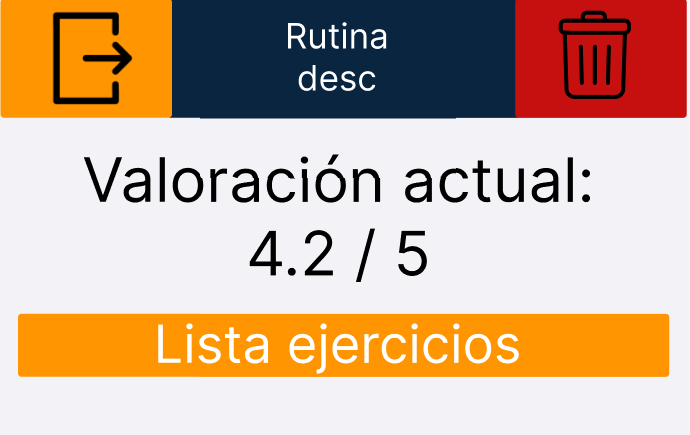
\includegraphics[width=0.6\textwidth]{fotos/Frame 49.png}
    \caption{Datos rutina no modificable}
    \label{fig:Datos rutina no modificable}
\end{figure}
\begin{figure}[H]
   \centering
    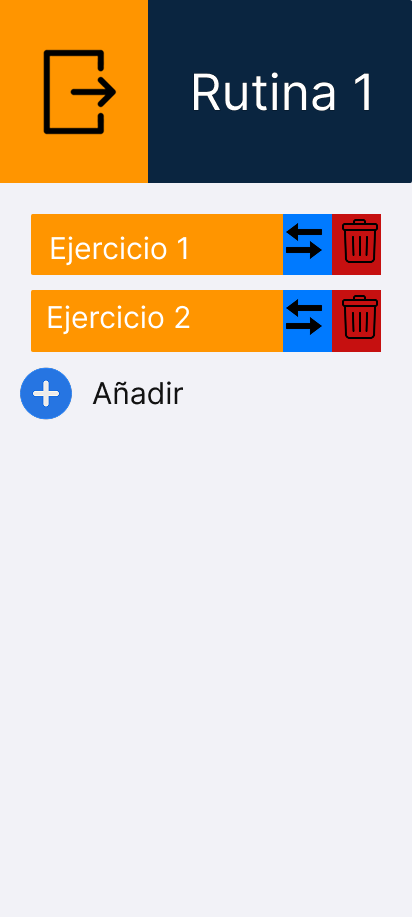
\includegraphics[width=0.6\textwidth]{fotos/Frame 50.png}
    \caption{Modificar ejericios rutina}
    \label{fig:Modificar ejericios rutina}
\end{figure}
\begin{figure}[H]
   \centering
    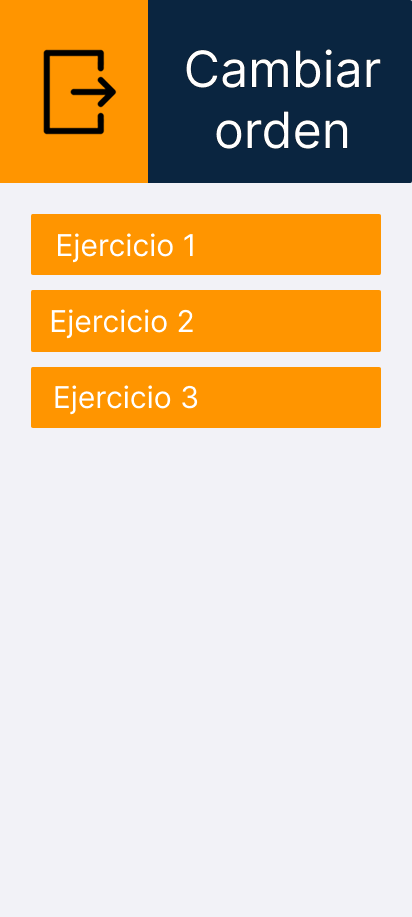
\includegraphics[width=0.6\textwidth]{fotos/Frame 51.png}
    \caption{Cambiar orden ejercicios rutina}
    \label{fig:Cambiar orden ejercicios rutina}
\end{figure}
\begin{figure}[H]
   \centering
    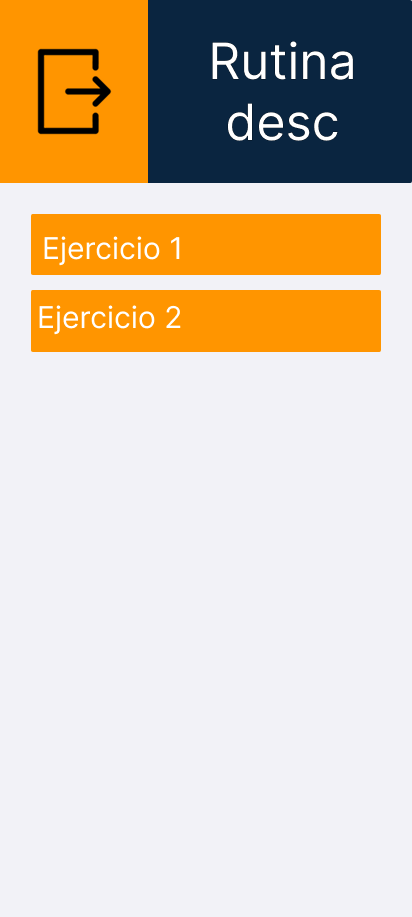
\includegraphics[width=0.6\textwidth]{fotos/Frame 52.png}
    \caption{Ejercicios rutina descargada}
    \label{fig:Ejercicios rutina descargada}
\end{figure}
\begin{figure}[H]
   \centering
    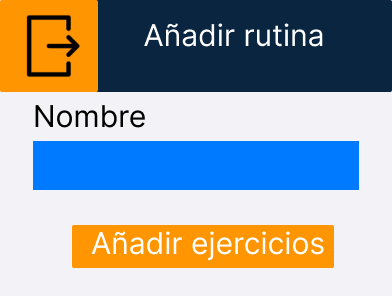
\includegraphics[width=0.6\textwidth]{fotos/Frame 65.png}
    \caption{Pop up crear rutinas}
    \label{fig:Pop up crear rutinas}
\end{figure}

\textbf{Mi perfil}

\begin{figure}[H]
   \centering
    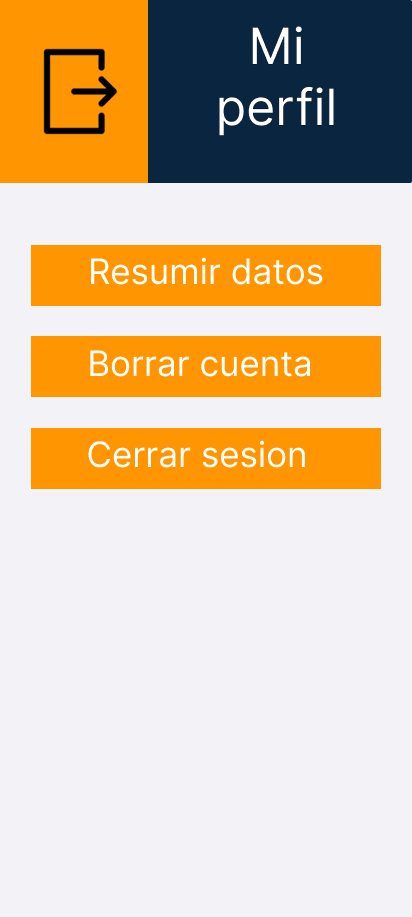
\includegraphics[width=0.6\textwidth]{fotos/Frame 36.png}
    \caption{Opciones de perfil usuario}
    \label{fig:Opciones de perfil usuario}
\end{figure}
\begin{figure}[H]
   \centering
    
\includegraphics[width=0.75\textwidth]{fotos/Frame 38.png}
    \caption{Pop up de confirmacion}
    \label{fig:Pop up de confirmacion}
\end{figure}
\begin{figure}[H]
   \centering
    
\includegraphics[width=0.75\textwidth]{fotos/Frame 39.png}
    \caption{Pop up de confirmacion resumir datos}
    \label{fig:Pop up de confirmacion resumir datos}
\end{figure}

\textbf{Buscar rutina para descargar}

\begin{figure}[H]
   \centering
    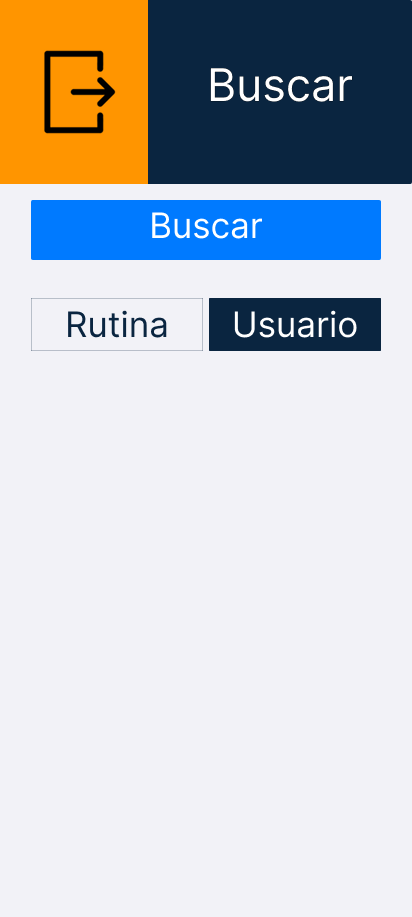
\includegraphics[width=0.6\textwidth]{fotos/Frame 53.png}
    \caption{Buscar usuario}
    \label{fig:Buscar usuario}
\end{figure}
\begin{figure}[H]
   \centering
    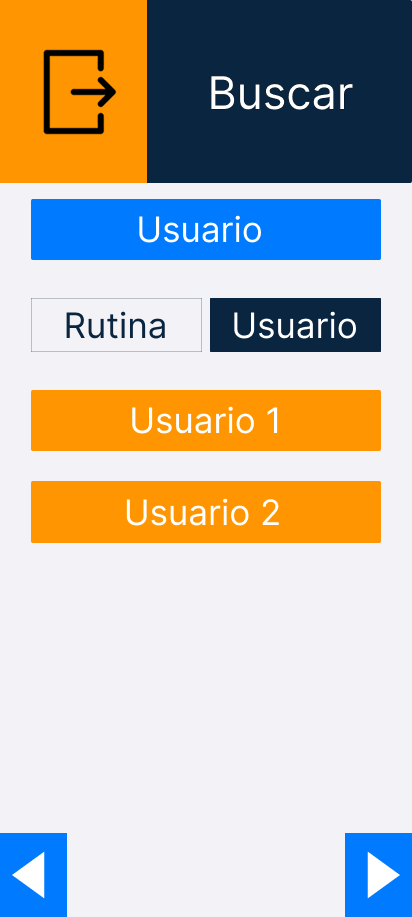
\includegraphics[width=0.6\textwidth]{fotos/Frame 54.png}
    \caption{Buscar usuario filtrado}
    \label{fig:Buscar usuario filtrado}
\end{figure}
\begin{figure}[H]
   \centering
    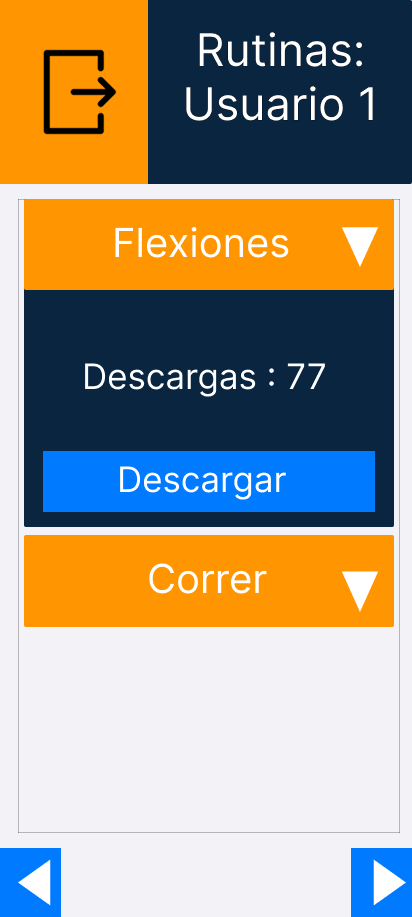
\includegraphics[width=0.6\textwidth]{fotos/Frame 56.png}
    \caption{Rutinas de un usuario}
    \label{fig:Rutinas de un usuario}
\end{figure}
\begin{figure}[H]
   \centering
    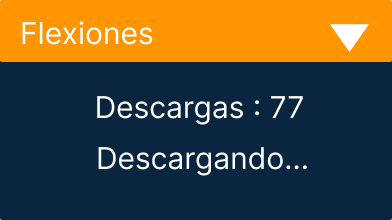
\includegraphics[width=0.6\textwidth]{fotos/Frame 57.png}
    \caption{Widget descargar rutina}
    \label{fig:Widget descargar rutina}
\end{figure}
\begin{figure}[H]
   \centering
    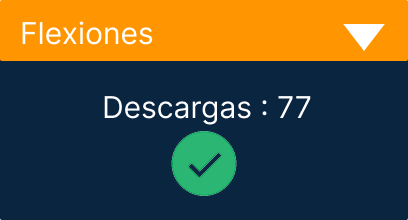
\includegraphics[width=0.6\textwidth]{fotos/Frame 58.png}
    \caption{Widget rutina descargada}
    \label{fig:Widget rutina descargada}
\end{figure}
\begin{figure}[H]
   \centering
    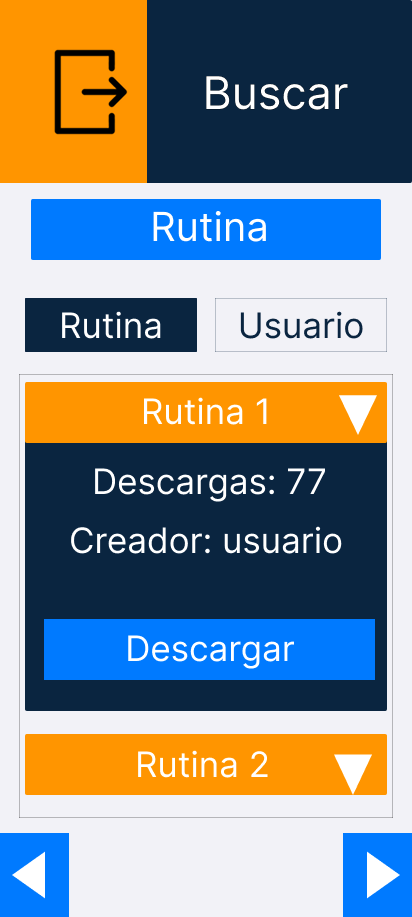
\includegraphics[width=0.6\textwidth]{fotos/Frame 59.png}
    \caption{Buscar rutinas por su nombre filtrada}
    \label{fig:Buscar rutinas por su nombre filtrada}
\end{figure}

\textbf{Entrenamiento (Una vez seleccionada una fecha en el calendario del menu principal saldría la siguiente ventana)}

\begin{figure}[H]
   \centering
    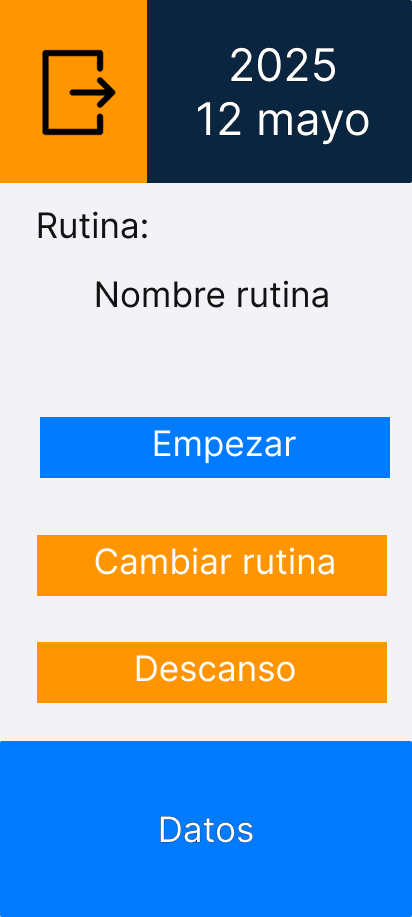
\includegraphics[width=0.6\textwidth]{fotos/Frame 26.png}
    \caption{Entrenamiento de un día determinado}
    \label{fig:Entrenamiento de un día determinado}
\end{figure}
\begin{figure}[H]
   \centering
    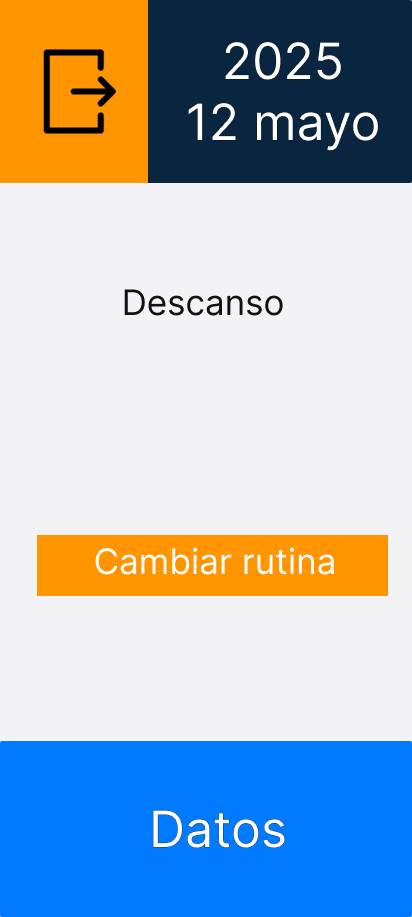
\includegraphics[width=0.6\textwidth]{fotos/Frame 27.png}
    \caption{Descanso en un día determinado}
    \label{fig:Descanso en un día determinado}
\end{figure}

Si seleccionamos datos de una fecha saldría esto
\begin{figure}[H]
   \centering
    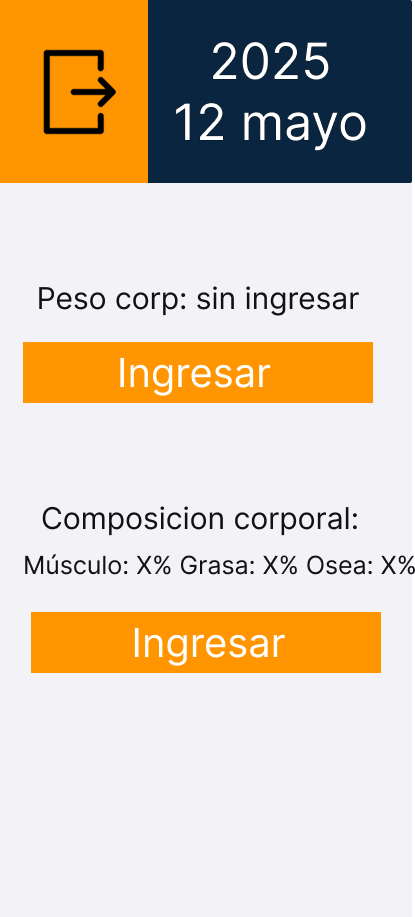
\includegraphics[width=0.6\textwidth]{fotos/Frame 29.png}
    \caption{Frame 29.png}
    \label{fig:Frame_29}
\end{figure}

La siguiente pantalla sale al comenzar el entrenamiento
\begin{figure}[H]
   \centering
    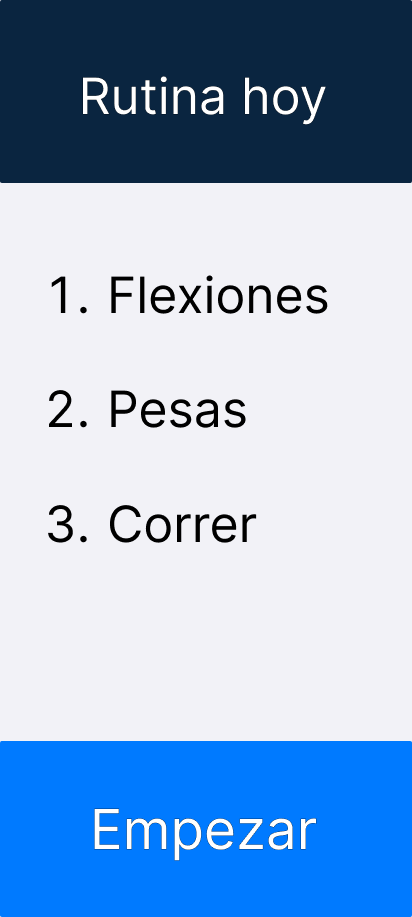
\includegraphics[width=0.6\textwidth]{fotos/Frame 1.png}
    \caption{Lista ejercicios del entrenamiento actual}
    \label{fig:Lista ejercicios del entrenamiento actual}
\end{figure}
\begin{figure}[H]
   \centering
    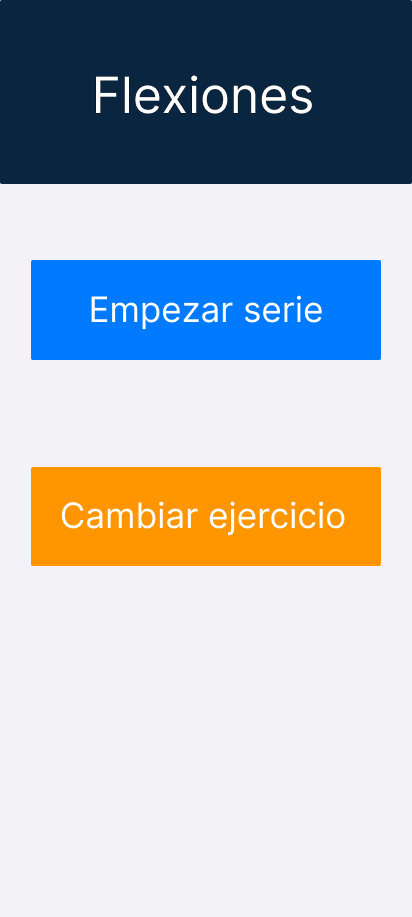
\includegraphics[width=0.6\textwidth]{fotos/Frame 2.png}
    \caption{Primera serie flexiones}
    \label{fig:Primera serie flexiones}
\end{figure}
\begin{figure}[H]
   \centering
    
\includegraphics[width=0.6\textwidth]{fotos/Frame 3.png}
    \caption{Realizando flexiones}
    \label{fig:Realizando flexiones}
\end{figure}
\begin{figure}[H]
   \centering
    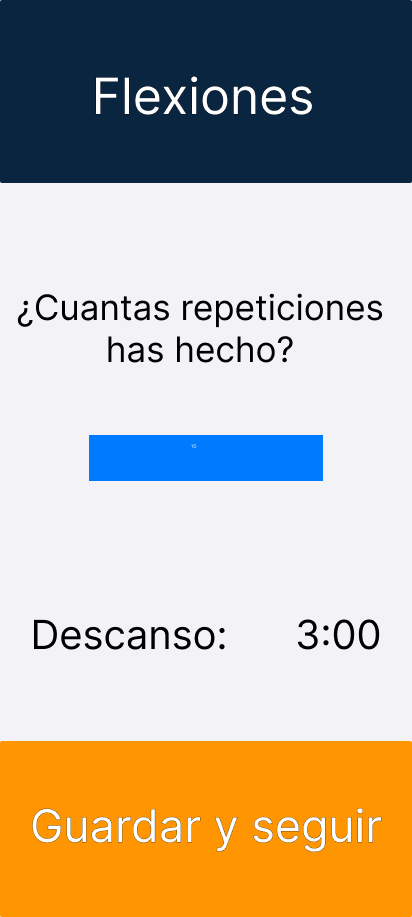
\includegraphics[width=0.6\textwidth]{fotos/Frame 4.png}
    \caption{Fin de la serie(Descanso no completado)}
    \label{fig:Fin de la serie(Descanso no completado)}
\end{figure}
\begin{figure}[H]
   \centering
    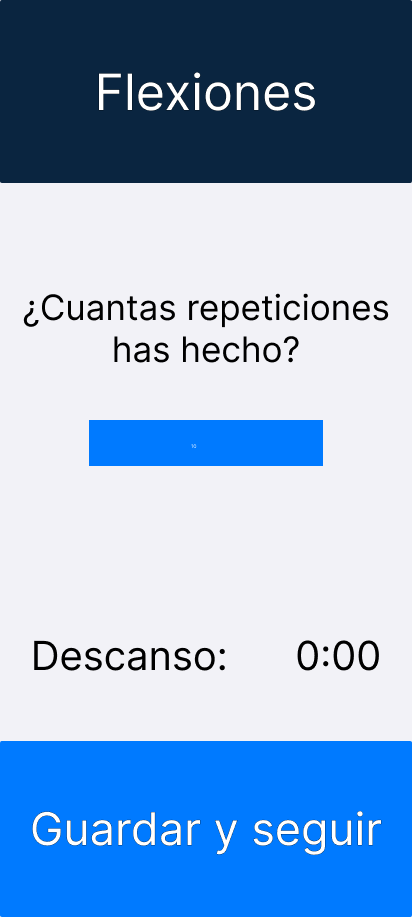
\includegraphics[width=0.6\textwidth]{fotos/Frame 5.png}
    \caption{Fin de la serie(Descanso completado)}
    \label{fig:Fin de la serie(Descanso completado)}
\end{figure}
\begin{figure}[H]
   \centering
    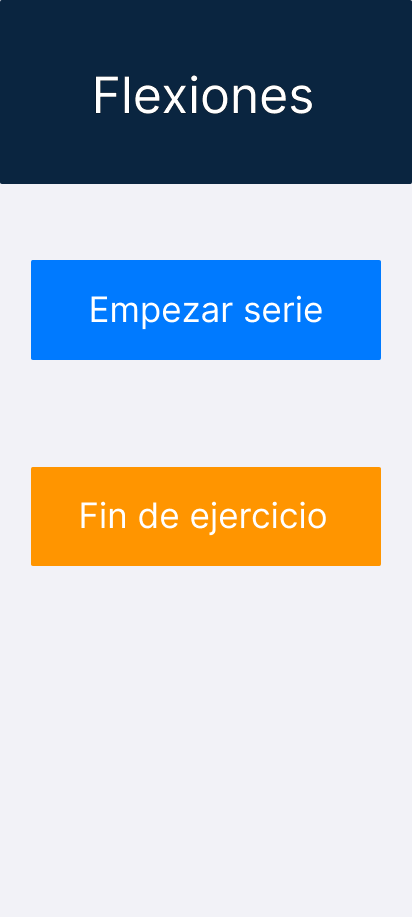
\includegraphics[width=0.6\textwidth]{fotos/Frame 62.png}
    \caption{Acabar ejercicio o añadir serie}
    \label{fig:Acabar ejercicio o añadir serie}
\end{figure}
\begin{figure}[H]
   \centering
    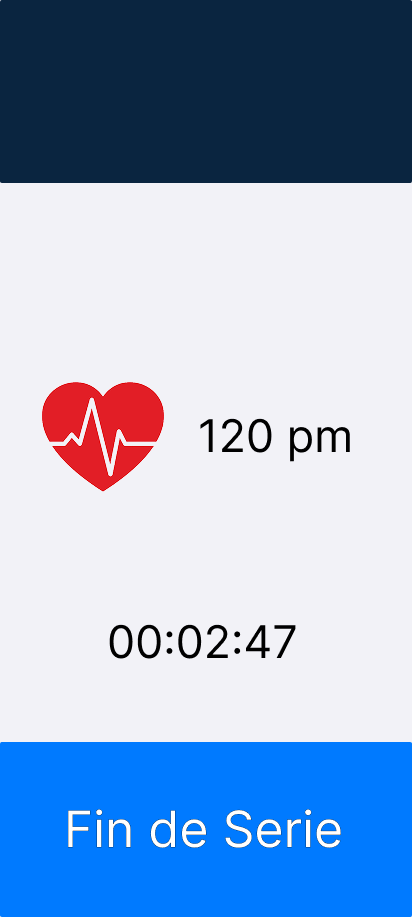
\includegraphics[width=0.6\textwidth]{fotos/Frame 60.png}
    \caption{Realizando ejercicio midiendo tiempo}
    \label{fig:Realizando ejercicio midiendo tiempo}
\end{figure}
\begin{figure}[H]
   \centering
    
\includegraphics[width=0.6\textwidth]{fotos/Frame 20.png}
    \caption{Fin entrenamiento}
    \label{fig:Fin entrenamiento}
\end{figure}
\begin{figure}[H]
   \centering
    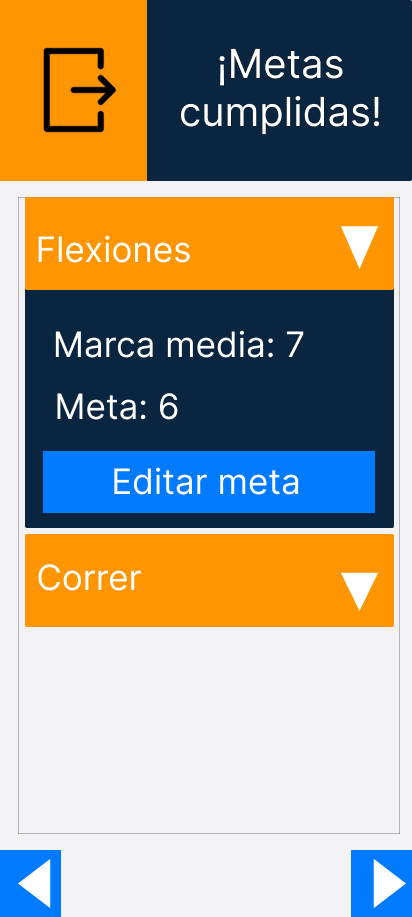
\includegraphics[width=0.6\textwidth]{fotos/Frame 37.png}
    \caption{Metas cumplidas}
    \label{fig:Metas cumplidas}
\end{figure}
\begin{figure}[H]
   \centering
    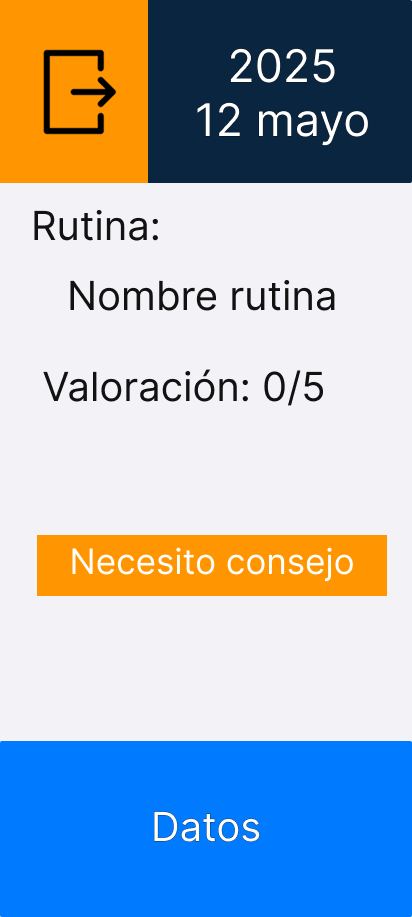
\includegraphics[width=0.6\textwidth]{fotos/Frame 31.png}
    \caption{Datos entrenamiento terminado}
    \label{fig:Datos entrenamiento terminado}
\end{figure}

El chat de la IA se abre cuando se le da a la opcion necesito consejo de un entrenamiento realizado
\begin{figure}[H]
   \centering
    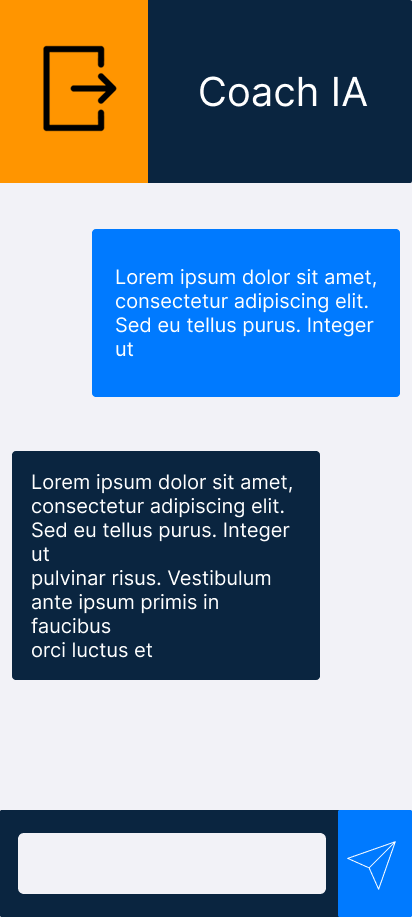
\includegraphics[width=0.6\textwidth]{fotos/Frame 32.png}
    \caption{Chat con IA}
    \label{fig:Chat con IA}
\end{figure}

Si le das a datos de un entrenamiento terminado
\begin{figure}[H]
   \centering
    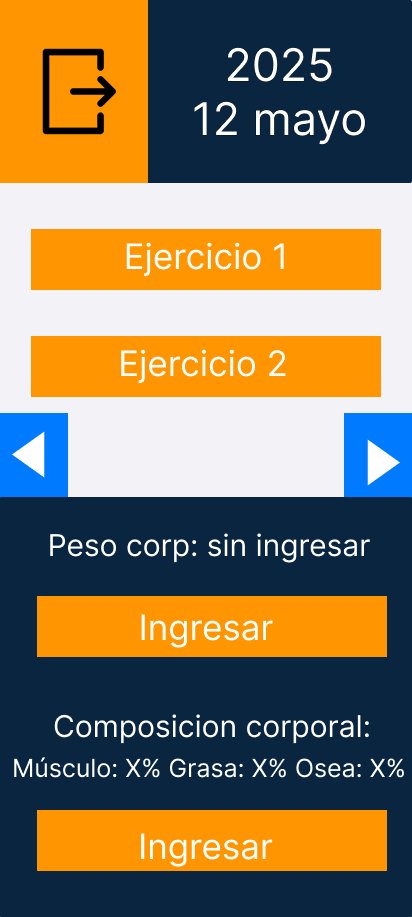
\includegraphics[width=0.6\textwidth]{fotos/Frame 33.png}
    \caption{Datos detallados entrenamiento terminado}
    \label{fig:Datos detallados entrenamiento terminado}
\end{figure}
\begin{figure}[H]
   \centering
    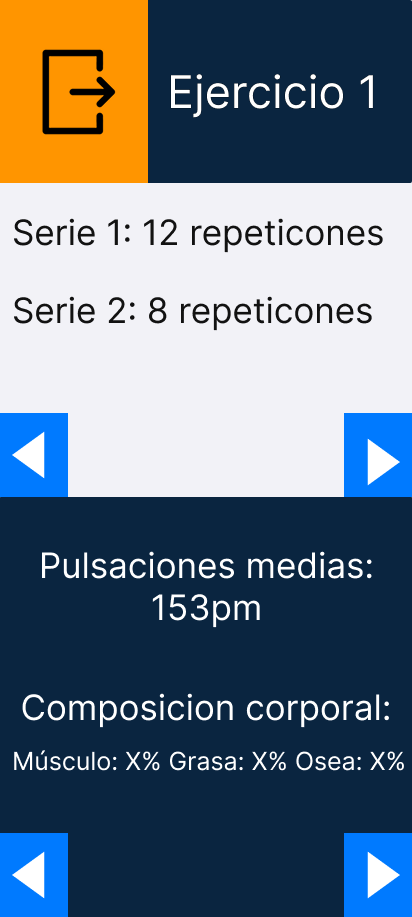
\includegraphics[width=0.6\textwidth]{fotos/Frame 35.png}
    \caption{Pop up datos de un ejercicio en entrenamiento}
    \label{fig:Pop up datos de un ejercicio en entrenamiento}
\end{figure}


Estos diseños pueden cambiar y sufrir alteraciones debido a los sprints reviews y correcciones de accesibilidad. De todas formas, cada cambio será informado con su motivo.

\subsubsection{Sprint Review 0}
Durante esta revisi\'on de sprint se realizaron mejoras de dise\~no, como la incorporaci\'on de iconos en todos los botones para mejorar la accesibilidad. Se revisaron los t\'itulos de las ventanas, cambiando aquellos que no eran lo suficientemente claros.

Adem\'as, se a\~nadieron nuevas historias al \textit{product backlog}:

\begin{itemize}
  \item SCRUM-42: Copiar rutina
  \item SCRUM-43: Añadir meta por parámetro
  \item SCRUM-44: Solicitar permiso al usuario antes de enviar datos a la IA
  \item SCRUM-45: Enviar datos del entrenamiento actual y anteriores a la IA
  \item SCRUM-46: Conectar/Desconectar con la IA
\end{itemize}

\subsection{Iteraci\'on 1}
Siendo la lista de la primera iteracion de la siguiente manera:

\begin{itemize}
    \item SCRUM-26: Buscar ejercicio en lista
    \item SCRUM-3: Insertar/Borrar/Modificar ejercicio de la lista de ejercicios
    \item SCRUM-27: Hacer la IU de la lista de ejercicios ELIMINAR
    \item SCRUM-28: Hacer la IU de creación de ejercicio ELIMINAR
    \item SCRUM-29: Pop up de confirmación
    \item SCRUM-30: Hacer IU de datos ejercicio ELIMINAR
\end{itemize}

\HU{
SCRUM-26: Buscar ejercicio en lista
}{
	\item Implementar la BD local
    \item Implementar algoritmo de búsqueda por nombre
   	\item Implementar boceto de IU \cref{fig:Lista ejercicios}
}{
	\item si no existe ejercicio buscado, no sale nada en pantalla
   	\item si existe ejercicio buscado, sale un acceso en pantalla
}
\HU{
SCRUM-3: Insertar/Borrar/Modificar ejercicio de la lista de ejercicios
}{
	\item Implementar la BD local
	\item Implementar las funciones para las consultas
	\item Implementar las funciones para las modificaciones
	\item Implementar las funciones para el borrado
	\item Implementar boceto de la IU \cref{fig:Datos ejercicio}, para borrar/modificar desde ahí
}{
	\item si se borra un ejercicio, no sale en la lista
	\item si se modifica, sale con los datos modificados
	\item si se inserta, sale en la lista el ejercicio
	\item se enseñan los datos del ejercicio de forma correcta
}
\HU{
SCRUM-43: Añadir meta por parámetro
}{
	\item Implementar la BD local
	\item Implementar las funciones para modificar metas
}{
	\item si existe una meta determinada para ese ejercicio y se quiere insertar una, sustituir la actual
}
\HU{
	SCRUM-29: Pop up de confirmación
}{
	\item Implementar la confirmación para que pueda ser usado en pantallas distintas
	\item Impelementar boceto de IU \cref{fig:Pop up de confirmacion}
}{
	\item si se ha seleccionado una opcion, se devuelve la opcion seleccionada
}

Dentro del SCRUM-3 tenemos subfuncionalidades, funciones pequeñas que componen la grande:

Durante esta iteraci\'on me familiaric\'e con Flutter y sus herramientas, como la base de datos local \textit{SQLite}.

\subsubsection{SQLite}
Es una base de datos ligera, autocontenida y de c\'odigo abierto. Usa el mismo lenguaje de consultas que SQL, lo que la hace ideal para la app. Adem\'as, permite transportar toda la BD en un \textit{.db}, lo cual puede facilitar funcionalidades como copias de seguridad descargables desde la nube.

\subsubsection{Estado de la BD local}

\begin{figure}[H]
   \centering
    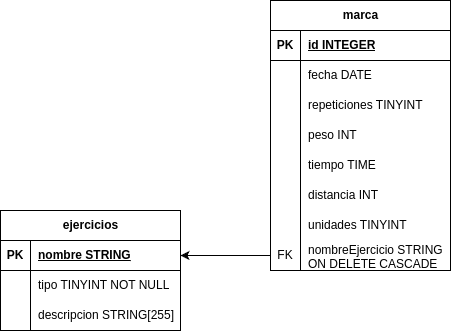
\includegraphics[width=\textwidth]{fotos/BDL iteracion 1.png}
    \caption{BD local iteracion 1}
    \label{fig:BD local iteracion 1}
\end{figure}

\subsubsection{Sprint Review 1}
Las primeras iteraciones tienden a ser m\'as lentas debido a la fase inicial del desarrollo. No se complet\'o la totalidad del sprint; qued\'o pendiente la subtarea de modificar ejercicio en la base de datos. Aun as\'i, las expectativas son positivas, ya que se espera un aumento en la velocidad de desarrollo. No obstante, en lo que se lleva  desarrollado han aparecido pocas problemáticas

\begin{figure}[h!]
  \centering
  \begin{minipage}[b]{0.45\textwidth}
    \centering
    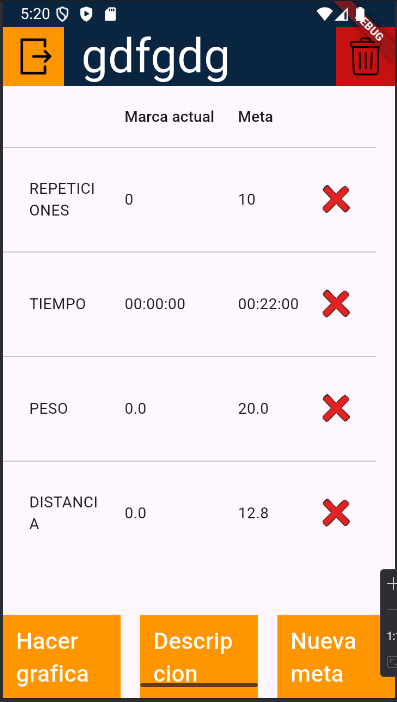
\includegraphics[width=\textwidth]{fotos/ejerciciosNueva.png}
    \caption{Pantalla nueva}
    \label{fig:pantalla_nueva}
  \end{minipage}
  \hfill
  \begin{minipage}[b]{0.45\textwidth}
    \centering
    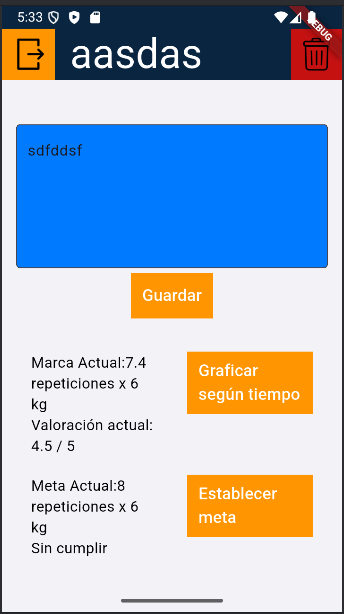
\includegraphics[width=\textwidth]{fotos/ejerciciosVieja.png}
    \caption{Pantalla antigua}
    \label{fig:pantalla_vieja}
  \end{minipage}
  \caption{Comparaci\'on entre la pantalla nueva y la anterior}
  \label{fig:comparacion_pantallas}
\end{figure}

\subsection{Iteraci\'on 2}
Esta iteraci\'on se centr\'o en el desarrollo del sistema de sesiones, la API de la aplicaci\'on, el backend b\'asico del servidor y la secci\'on de rutinas.

\begin{itemize}
  \item SCRUM-21 Crear/Borrar mi usuario
  \item SCRUM-23 Iniciar/Cerrar sesión
  \item SCRUM-6 Insertar/Borrar/Modificar rutina
  \item SCRUM-4 Buscar rutina en la lista del usuario
  \item SCRUM-31 Crear IU de la lista de las rutinas ELIMINAR
  \item SCRUM-32 Crear IU de pantalla inicial ELIMINAR
  \item SCRUM-33 Implementar menú principal
  \item SCRUM-34 Crear IU datos rutinas ELIMINAR
  \item SCRUM-35 IU lista ejercicios de rutina modificable ELIMINAR
  \item SCRUM-36 Crear IU para crear rutina ELIMINAR
\end{itemize}

\HU{
SCRUM-33 Implementar menú principal
}{
	\item Implementar el boceto IU \cref{fig:Menu principal}
	\item Añadir accesos a las funcionalidades actuales
}{
	\item si la funcionalidad seleccionada no está implementada, no hacer nada
	\item si la funcionalidad seleccionada está implementada, desplegar ventana de dicha funcionañidad
}
\HU{
SCRUM-21 Crear/Borrar mi usuario
}{
	\item Implementar bocetos de IU \cref{fig:Crear cuenta 1} ,\cref{fig:Crear cuenta 2}, \cref{fig:Pagina inicial} y la parte necesaria de \cref{fig:Opciones de perfil usuario}
	\item Implementar funciones de inserccion y borrado en el backend
}{
	\item si el usuario que se quiere crear ya existe, informar y pedir que se rellenen los credenciales otra vez
	\item si el usuario que se quiere crear no existe, crear usuario y pasar a la siguiente pantalla
	\item si cualquier dato requerido está en un formato incorrecto ,informar al usuario para que vuelva a rellenar estos
	\item si todos los datos están en el formato correcto ,seguir con la creación del usuario
	\item si se ha creado exitosamente el usuario, volver a la pantalla inicial
	\item si se borra el usuario, borrar el token en el dispositvo y sus credenciales en el backend
}
\HU{
SCRUM-23 Iniciar/Cerrar sesión
}{
	\item Implementar el boceto IU \cref{fig:Inicio de sesion} y parte necesaria de \cref{fig:Opciones de perfil usuario}
	\item Implementar función de consulta en el backend
}{
	\item si el usuario con esa contraseña no existe, informar al usuario
	\item si el usuario con esa contraseña existe, devolver un token para su guardado y guardar usuario 
	\item si el usuario quiere cerrar sesión, borrar token y nombre del usuario del dispositivo y volver a la pantalla inicial \cref{fig:Pagina inicial}
}
\HU{
SCRUM-4 Buscar rutina en la lista del usuario
}{
	\item Implementar IU del boceto \cref{fig:Lista rutinas}
	\item Implementar lo necesario en la BD local
	\item Implementar algorítmo de búsqueda
	\item Implementar acceso a la rutina seleccionada
}{
	\item si no existe la rutina buscada, no enseñar acceso en pantalla
	\item si existe la rutina buscada, enseñar acceso en pantalla
}
\HU{
SCRUM-6 Insertar/Borrar/Modificar rutina
}{
	\item Implementar las insercciones en para la BD local
	\item Implementar los borrados para la BD local
	\item Implementar las modificaciones para la BD local
}{
	\item si se hace una insercción, que el elemento insertado sea visible en la lista de ejercicios
	\item si se hace un borrado, que el elemento desaparezca de la lista
	\item si se hace una modificación, que se hagan visibles los cambios al momento
	\item si hay algún fallo en alguna de estas operaciones, informar al usuario con el motivo
}
\subsubsection{Sistema de sesiones}
Se implement\'o un sistema de autenticaci\'on basado en tokens. Cuando el usuario verifica su identidad, recibe un token que se guarda en el dispositivo y se usa para validar el acceso posterior. Esto evita que usuarios no autorizados suban contenido haci\'endose pasar por otros.

El backend est\'a desarrollado en \textit{Node.js} y utiliza una base de datos SQL para gestionar las contrase\~nas de los usuarios. Este mismo backend se usar\'a para las funcionalidades de las siguientes iteraciones.

\subsubsection{API de la app}
La comunicaci\'on entre la app y el servidor se realiza mediante peticiones HTTP. En el futuro, estas podr\'an migrarse a HTTPS para proteger operaciones sensibles. Por ahora se mantiene HTTP para facilitar el depurado.

\subsubsection{Cambios importantes}
Se redise\~n\'o la implementaci\'on de las pantallas con listas. En lugar de una \'unica clase con condiciones para la visibilidad de elementos, se opt\'o por crear clases espec\'ificas para cada tipo de lista.

\textbf{Ventaja:} El c\'odigo es m\'as limpio, escalable y modular. Si hay que modificar un tipo de lista, los dem\'as no se ven afectados.

\subsubsection{Sprint Review 2}
Se sugirieron mejoras menores como el ajuste de tama\~nos e iconos en los botones de la secci\'on de creaci\'on de rutinas.

Tambi\'en se modific\'o la funcionalidad de compartir rutinas. Ahora todas son modificables, eliminando la distinci\'on entre rutinas descargadas (antes no modificables) y creadas (modificables). Esto mejora la experiencia del usuario: si desea volver a una rutina original, simplemente la puede volver a buscar y descargar.

Se cumplieron todas las funcionalidades en este sprint.

\subsubsection{Estado de la BD local}

\begin{figure}[H]
   \centering
    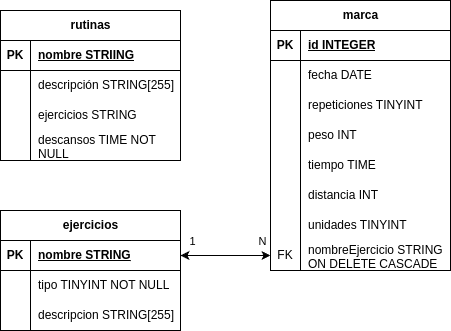
\includegraphics[width=\textwidth]{fotos/BDL iteracion 2.png}
    \caption{BD local iteracion 2}
    \label{fig:BD local iteracion 2}
\end{figure}

\subsubsection{Estado de la BD backend}

\begin{figure}[H]
   \centering
    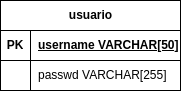
\includegraphics[width=0.7\textwidth]{fotos/BD be iteracion 2.png}
    \caption{BD backend iteracion 2}
    \label{fig:BD backend iteracion 2}
\end{figure}

\subsection{Iteraci\'on 3}
Esta iteraci\'on se centr\'o en desarrollar la funcionalidad para compartir rutinas entre usuarios, incluyendo la subida, visualizaci\'on y descarga de rutinas. Adem\'as, se comenz\'o a implementar la funcionalidad de resumen de datos para optimizar el uso de la memoria local.

\begin{itemize}
  \item SCRUM-2 Establecer peso objetivo
  \item SCRUM-37 Crear IU del perfil del usuario ELIMINAR
  \item SCRUM-42 Copiar rutina
  \item SCRUM-10 Enseñar datos de una rutina a descargar
  \item SCRUM-11 Compartir mi rutina
  \item SCRUM-39 Buscar rutinas para descargar
  \item SCRUM-9 Revisar datos para ver si el descanso es necesario
  \item SCRUM-22 Resumir datos
  \item SCRUM-40 IU del pop up de resumir datos ELIMINAR
  \item SCRUM-41 IU desplegable rutina ELIMINAR
\end{itemize}
\HU{
SCRUM-2 Establecer peso objetivo
}{
	\item Implementar la parte necesaria de \cref{fig:Opciones de perfil usuario}
	\item Implementar el almacenaje de ese peso objetivo
}{
	\item si el peso objetivo está en el formato correcto, guardar
	\item si el peso objetivo no está en el formato correcto, enseñar una alerta para su corrección
}
\HU{
SCRUM-11 Compartir mi rutina
}{
	\item Implementar la BD en el backend
	\item Implementar funciones de inserción en la API
}{
	\item si la rutina no contiene ejercicios, no permitir su subida al servidor
	\item si la rutina contiene ejercicios, permitir la subida al servidor
}
\HU{
SCRUM-39 Buscar rutinas para descargar
}{
	\item Implementar funciones de consultas en la API
	\item Implementar IU de busqueda de rutinas por usuario creador y por nombre de rutina
}{
	\item si busco un usuario que no existe, no se muestra ningún acceso en la IU
	\item si busco un usuario existente, se muestra su acceso en la IU
	\item si busco una rutina que no existe, no se muestra ningún acceso en la IU
	\item si busco una rutina existente, se muestra su acceso en la IU
}
\HU{
SCRUM-10 Enseñar datos de una rutina a descargar
}{
	\item Implementar el IU pop up
	\item Implementar las funciones de consulta en la API
	\item Implementar las funciones de inserción en la BD local
}{
	\item si se va a descargar la rutina y el usuario tiene en el dispositivo otra con el mismo nombre, un algorítmo resolverá este problema
	\item si se va a descargar la rutina y el usuario no tiene en el dispositivo otra con el mismo nombre, descargar normalmente
}
\HU{
SCRUM-42 Copiar rutina
}{
	\item Añadir al boceto IU de datos rutina \cref{fig:Datos rutina modificable} esta funcionalidad
	\item Implementar la IU resultante de la tarea anterior
	\item Implementar las consultas e inserciones necesarias en la BD local
}{
	\item si hay algún problema por coincidencia de nombres, un algorítmo resolverá este problema
	\item si no hay algún problema por coincidencia de nombres, copiar
}

Durante la realización de estas tareas de usuario, se dió notoriedad a que las historias restantes de este sprint (SCRUM-9 Revisar datos para ver si el descanso es necesario y SCRUM-22 Resumir datos) no pueden ser implementadas en este punto del desarrollo. Se pospondrán para su futura implementación.

\subsubsection{Funcionalidad descartada}

Se ha decidido, descartar una funcionalidad, en concreto el SCRUM-9 (Revisar datos para ver si el descanso es necesario), dado porque necesitaría los datos de un smartwatch y ha sido una funcionalidad previamente descartada.

También se ha descartado SCRUM-42 (Copiar rutina), dado que aporta poco valor a la app.

\subsubsection{Peso objetivo}
El peso objetivo es una meta que define el usuario y se almacena en memoria. Esta meta se representar\'a en la gr\'afica de evoluci\'on del peso del usuario, y se generar\'a una alerta cuando dicha meta sea alcanzada. La visualizaci\'on a\'un no ha sido implementada completamente.

\subsubsection{Cambios durante el desarrollo}
Durante esta iteraci\'on surgieron cambios en la forma de visualizar y gestionar las rutinas compartidas y almacenadas:

\begin{itemize}
  \item Ahora, al descargar una rutina, se a\~nade el nombre del creador al nombre de la rutina, facilitando la distinci\'on entre rutinas propias y descargadas.
  \item Cuando hay conflicto de nombres al crear una rutina, se genera un nombre alternativo del tipo \texttt{Nombre(n)}, siendo \texttt{n} un n\'umero incremental.
  \item Se ha implementado un selector entre ``Mis rutinas'' y ``Compartidas'' para facilitar la visualizaci\'on de las rutinas subidas a la nube por el usuario.
  \item Se reemplaz\'o el filtro integrado en la ventana de b\'usqueda por un selector emergente que permite buscar rutinas por nombre o por nombre de usuario.
  \item La interfaz de descarga y visualizaci\'on de rutinas ahora es un cuadro emergente (pop-up) en lugar de un desplegable.
\end{itemize}

\subsubsection{Imprevistos y problemas en el desarrollo}
Se identificaron dos errores principales de planificaci\'on:

\begin{description}
  \item[Error 1:] Se planific\'o implementar la funcionalidad de resumir datos sin haber completado la obtenci\'on de datos. \\ \textbf{Soluci\'on:} Replanificar los sprints.
  \item[Error 2:] Se subestim\'o la complejidad del sistema de rutinas compartidas, especialmente en la resoluci\'on de conflictos de nombres. \\ \textbf{Soluci\'on:} Aplicar nombres combinados (nombre + creador + copia) en memoria local e identificadores \textit{autoincrementales} en la nube.
\end{description}

\subsubsection{Valor a\~nadido a la app}
Los imprevistos y problemas surgidos durante el desarrollo han permitido detectar \textit{bugs}, errores de dise\~no y carencias funcionales que de otro modo podr\'ian haber pasado desapercibidos. Gracias a ello, se han podido proponer nuevas funcionalidades y mejorar las ya existentes, lo cual contribuye significativamente a aumentar la calidad global de la aplicaci\'on.

Algunas de las funcionalidades propuestas como mejora son:

\begin{itemize}
  \item Verificar el token del usuario antes de permitir la subida de rutinas, para evitar suplantación.
  \item Al seleccionar la opci\'on de borrar usuario del dispositivo, eliminar tambi\'en la base de datos local asociada.
  \item Crear una base de datos local independiente para cada nuevo usuario creado en un dispositivo.
  \item Posibilidad de editar el nombre de una rutina.
  \item Marcar los ejercicios eliminados con una \textit{flag}, para evitar que se inicien rutinas que los contengan.
  \item Marcar a los usuarios permanentemente eliminados con una \textit{flag}, para proceder a eliminarlos en los dispositvos.
\end{itemize}

Estas funcionalidades est\'an pensadas para aportar mayor \textbf{seguridad}, \textbf{integridad} y \textbf{calidad} al producto final.

\subsubsection{Base de datos del backend}
La base de datos utilizada en el backend está basada en \textit{MySQL}. En ella se almacenan los usuarios junto con sus contraseñas, así como los ejercicios y las rutinas. Las rutinas están vinculadas al usuario que las creó, y los ejercicios se asocian a las rutinas a las que pertenecen. Si un usuario decide eliminar su cuenta de forma permanente, las rutinas y ejercicios relacionados se eliminarán en cascada.

Al descargar una rutina, los ejercicios asociados se guardan en la memoria local del usuario como si fueran de su propiedad. Es decir, el usuario puede modificarlos libremente sin restricciones.

\subsubsection{Estado BD local}

No ha habido cambios respecto a la iteración anterior

\subsubsection{Estado BD backend}

\begin{figure}[H]
   \centering
    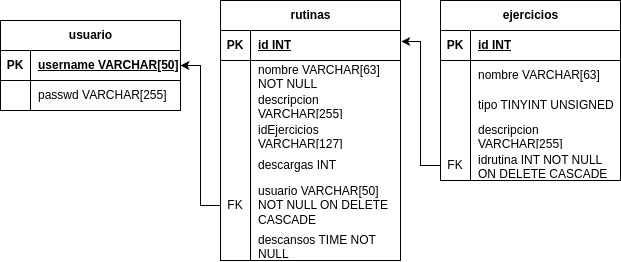
\includegraphics[width=\textwidth]{fotos/BD be iteracion 3.png}
    \caption{BD backend iteracion 3}
    \label{fig:BD be iteracion 3}
\end{figure}

\subsubsection{Sprint Review 3}

En esta review se estuvo debatiendo si quitar las funcionalidades relacionadas con el smartwatch, por cuestiones de tiempo, ya que con las funcionalidades añadidas en el capitulo anterior se va ajustando el plazo.

En esta iteración se tenía pensado implementar la funcionalidad de resumir los datos, no obstante, al no tener implementada la parte en la que guardo las marcas de los entrenamientos, no puedo trabajar en esa funcionalidad. Por lo tanto, se ha pospuesto para la próxima iteración. También se le dió el visto bueno a la implementación de las funcionalidades previamente expuestas durante el desarrollo.

También, debido al querer hacer la app accesible se ha decidido sustituir los pop ups por pantallas normales, dado que los pop ups son un gran problema para este objetivo, debido a que un usuario puede hacerlo desaparecer este tocando fuera del area en pantalla de este.

\subsection{Iteraci\'on 4}

En esta iteración se tiene pensado implementar la funcionalidad del calendario, donde el usuario podrá ver su planificación y acceder a sus marcas. Por otro lado, también se implementarán las funcionalidades nuevas del sprint anterior y las nuevas pantallas.

\begin{itemize}
	  \item SCRUM-39 Detectar metas cumplidas en los ejercicios despues del entrenamiento
	  \item SCRUM-1 Registrar peso por día
	  \item SCRUM-19 Realizar el flujo del entrenamiento
	  \item SCRUM-44: Implementar calendario
\end{itemize}

\HU{
SCRUM-44: Implementar calendario
}{
	\item Implementar la IU e insertarla en el menu principal \cref{fig:Menu principal}
	\item Implementar en la BD local
	\item Implementar funciones de inserción en BD local
	\item Implementar funciones de consulta en BD local
	\item Implementar funciones de borrado en BD local
	\item Implementar un acceso para ver los datos registrados sobre un día en concreto
}{
	\item si un día no tiene una rutina asignada, se considera descanso
	\item si un día tiene una rutina asignada, no hay marcas registradas y el día ya ha pasado, no se enseñará información, ya que se considera no entrenado
	\item si un día tiene una rutina asignada, no hay marcas registradas pero es hoy, se enseñará un acceso para empezar el entrenamiento, se considera que el usuario todavía no ha entrenado
	\item si un día tiene una rutina asignada, pero es futuro, no se enseñará un acceso para empezar el entrenamiento
	\item si un día tiene una rutina asignada y hay marcas registradas sea el día actual o pasado, se mostrará información de las marcas, sin acceso a entrenamiento
}
\HU{
SCRUM-19 Realizar el flujo del entrenamiento
}{
	\item Implementar IU de las pantallas de entrenamientos(de la \cref{fig:Lista ejercicios del entrenamiento actual}  a la \cref{fig:Fin entrenamiento})
	\item Implementar una clase que controle el cambio entre distintas pantallas y el guardado de marcas
}{
	\item si la rutina asignada para un día, no tiene ejercicios y se desea iniciar el entrenamiento, se muestra por pantalla una alerta y no se permite continuar con el entrenamiento
	\item si la rutina asignada para un día, tiene ejercicios, comienza el recorrido entre IUs
	\item si es la primera serie de un ejercicio, no se permite terminar el ejercicio
	\item si no es la primera serie de un ejercicio, se permite terminar el ejercicio
	\item si acaba una serie, no se permitirá acabar el ejercicio o continuar con este hasta que termine el tiempo de descanso que se muestra en pantalla
	\item si finaliza el último ejercicio de la lista, fin del entrenamiento, se devuelve al usuario al menú principal
}
\HU{
SCRUM-39 Detectar metas cumplidas en los ejercicios despues del entrenamiento
}{
	\item Implementar bocetos de IU \cref{fig:Metas cumplidas}
	\item Implementar lógica para comparar marcas y metas despues de acabar el entrenamiento en la clase que controla el flujo del entrenamiento
}{
	\item si en un ejercicio no se ha cumplido la meta, no se enseña nada
	\item si en un ejercicio cumplimos una meta, se enseña en que ejercicio se cumplió la meta
}
\HU{
SCRUM-1 Registrar peso por día
}{
	\item Implementar boceto de IU \cref{fig:Datos detallados entrenamiento terminado}
	\item Implementar en BD local
	\item Implementar funciones de inserción
	\item Implementar funciones de consulta
	\item Implementar lógica para determinar si un usuario quiere subir o bajar de peso
}{
	\item si se introduce algún dato como formato incorrecto, se muestra una alerta por pantalla
	\item si se introducen los datos en formato correcto, se guarda
}

En esta iteración hay pocas funcionalidades commparadas con otras, porque el flujo del entrenamiento es una funcionalidad muy grande. A parte se añade esta funcionalidad que también se va a realizar en esta iteración, SCRUM-44 Implementar calendario.

\subsubsection{Paquete tableCalendar}

Es un paquete de flutter, que permite implementar y customizar un calendario, de forma fácil y rápida. También permite trabajar con información para reflejarla en las fechass del calendario.

\begin{figure}[h!]
    \centering
    \includegraphics[width=0.45\textwidth]{fotos/PantallaCalendario.png}
    \caption{Pantalla Calendario}
    \label{fig:Pantalla Calendario}
\end{figure}

Existen varios formatos de calendario preimplementados, que cambian el numero de dias en pantalla, se escogió este porque es el que menos problemas da en pantalla y más cómodo para las interacciones que busca el usuario.

\subsubsection{Pantallas cambiadas por pop ups}

La solución que se ha dado para que este problema no quite mucho tiempo de desarrollo es la siguiente, reciclar todo el contenido posible del interior de los pop ups y plasmarlo tal cual en una pantalla. Dado que los diseños implementados eran buenos, quitando algún fallo que puedan dar por este cambio de formato.

Los pop ups que se cambiaron son los siguientes:

\begin{itemize}
	\item Los pop ups de confirmacion
	\item Crear ejercicios
	\item Modificar ejercicios
	\item Nueva meta en un ejercicio
	\item Crear rutinas
	\item Modificar rutinas
	\item Modificar ejercicios de una rutina
	\item Información de una rutina a descargar
	\item Modificar informacion del perfil del usuario
\end{itemize}

Por consecuencia las futuras funcionalidades en la que se mencionan los pop ups, pasaran a ser pantallas completas.

\subsubsection{Cambios en el backend}

Los cambios en el backend están relacionados con las siguientes funcionalidades propuestas en la iteracion anterior:

\begin{itemize}
	\item Cambio 1: Verificar el token del usuario antes de permitir la subida de rutinas, para evitar suplantación.
  	\item Cambio 2: Marcar a los usuarios permanentemente eliminados con una \textit{flag}, para proceder a eliminarlos en los dispositvos.
\end{itemize}

Cambio 1: la solución implementada es la siguiente, a todas las funciones que puedan ser potencialmente victimas de una suplantación(via peticion normal de http), se les ha añadido un middleware, una función que se ejecuta antes para verificar el token. Express.js permite implementar esto rapidamente

Cambio 2: de primeras se pensó en usar una flag, pero finalmente para evitar perdida de rendimiento al momento de que el usuario realize un entrenamiento(que es cuando en un principio se tenía pensado borrar el ejercicio), se optó por modificar la lista de ejercicios de la rutina al momento de borrar el ejercicio. El número de consultas iba a ser el mismo, pero se ahorra memoria, ya que no añadimos una columna más a la tabla de ejercicios

\subsubsection{Flujo entrenamiento}

Para acaparar esta funcionalidad, se ha implementado una clase aparte encargada del desarrollo de esta parte de la app. Se ha decidido así ya que es una lógica más compleja y es conveniente tenerla separada de la IU.

Esta clase, solo se puede crear de forma util llamando a un método estático de la propia clase (se hace así ya que necesita hacer operaciones asíncronas para obtener los datos necesarios), este método estático me devuelve la instancia con la que voy a trabajar. Se llama al método ejecutar de la instancia creada y sola se encarga de mostrar las pantallas al usuario, guardar los datos y de comparar las metas que se propuso el usuario.

Aquí un diagrama de actividades que explica la tarea de esta clase:

\begin{figure}[H]
    \centering
    \includegraphics[width=0.75\textwidth]{tablas/FlujoEntrenamiento.png}
    \caption{Flujo entrenamiento}
    \label{fig:Flujo entrenamiento}
\end{figure}

\subsubsection{Estado de la BD local}

\begin{figure}[H]
    \centering
    \includegraphics[width=\textwidth]{fotos/BDL iteracion 4.png}
    \caption{BD local iteración 4}
    \label{fig:BDL iteracion 4}
\end{figure}

\subsubsection{Estado BD backend}

No sufrió cambios respecto a la iteración anterior

\subsubsection{Sprint review 4}

En esta review se ha propuesto que despues de los entrenamientos se les enseñe a los usuarios las metas que tenían establecidas siempre, aunque no la hayan superado, evitando siempre el feedback negativo al usuario.

\subsection{Iteraci\'on 5}

Debido a retrasos y problemas durante el desarrollo esta será la última iteración, que se dedicará a la implementación de gráficas para representar los datos requeridos por el usuario. Dado al tiempo limitado que se posee la implementación de la IA se aplazará al máximo e incluso siendo posible su descarte.